\documentclass[twoside,twocolumn]{article}
    \usepackage[a4paper, left=2cm, right=2cm]{geometry} % A4 paper size and thin margins
    \usepackage[sc]{mathpazo} % Use the Palatino font
    \usepackage[T1]{fontenc} % Use 8-bit encoding that has 256 glyphs
    \usepackage{microtype} % Slightly tweak font spacing for aesthetics
    \usepackage[english]{babel} % Language hyphenation and typographical rules
    \usepackage{booktabs} % Horizontal rules in tables
    \usepackage{enumitem} % Customized lists
    \usepackage{xcolor} % Required for specifying custom colours
    \usepackage[utf8]{inputenc} % Required for inputting international characters
    \usepackage{parskip}
    \usepackage{graphicx}
    \usepackage{hyperref}
    \usepackage{pdfpages}
    \usepackage{amsmath}
    \usepackage{esvect}
    \usepackage{listings}
    \usepackage[title]{appendix}
    \hypersetup{
        colorlinks=true,
        linkcolor=blue,
        filecolor=magenta,      
        urlcolor=cyan,
    }
    \urlstyle{same}
    \setlength{\parindent}{15pt}
    \setlist[itemize]{noitemsep} % Make itemize lists more compact
    \makeatletter
    \newcommand*{\rom}[1]{\expandafter\@slowromancap\romannumeral #1@}
    \g@addto@macro{\UrlBreaks}{\UrlOrds}
    \makeatother

    \title{\LARGE \bf
    Principal Component Analysis of Physical Systems
    }
    
    \author{ \parbox{3 in}{\centering Chongyi Xu \\
             University of Washington\\
             AMATH 482/582 Winter Quarter 2018\\
             {\tt\small chongyix@uw.edu}}
    }

    \begin{document}
    \maketitle

    %----------------------------------------------------------------------------------------
    %	ARTICLE CONTENTS
    %----------------------------------------------------------------------------------------
    \begin{abstract}

    The principal component analysis (PCA) is a kind of algorithms in biometrics. It is a statistics 
    technical and used orthogonal transformation to convert a set of observations of possibly correlated 
    variables into a set of values of linearly uncorrelated variables. PCA also is a tool to reduce 
    multidimensional data to lower dimensions while retaining most of the information. It covers standard 
    deviation, covariance, and eigenvectors.
        
    \end{abstract}

    \linespread{1.05} % Line spacing - Palatino needs more space between lines
    %------------------------------------------------
    \section{Introduction and Overview}
    \subsection{Introudction}
    In real life, it always happens that we would like to konw about a certain physical phenomena. However, 
    without relative knowledge or theorm, it is hard to understand the phenomena by oneself. In order to 
    understand our world, we sometimes tried to performe a certain experiment that could reproduce the real-life 
    situation and recorded the data to study for it. And since we do not know the concept (or theorm) about the 
    phenomena, the data we collected from experiments will always be redundant and noisy. The principal component
    analysis (PCA) provides statistical helps to rearrange and optimize the data such that the result we got from
    the data could be more convincing and effective.

    %------------------------------------------------
    \subsection{Overview}
    We are going to explore 4 cases to illustrate various aspects of PCA and its practical usefulness and the effects 
    of noise on the PCA algorithm.
    \begin{itemize}
        \item Ideal case
        \item Noisy case
        \item Horizontal displacement
        \item Horizontal displacement and rotation
    \end{itemize}
    We have the videos for every cases from 3 different cameras and the purpose is to understand the system. 
    %------------------------------------------------
    \section{Theoretical Background}
    PCA was invented in 1901 by Karl Pearson, as an analogue of the principal axis theorem in mechanics; 
    it was later independently developed and named by Harold Hotelling in the 1930s. Depending on the field 
    of application, it is also named the discrete Karhunen–Loève transform (KLT) in signal processing, the 
    Hotelling transform in multivariate quality control, proper orthogonal decomposition (POD) in mechanical 
    engineering, singular value decomposition (SVD) of X (Golub and Van Loan, 1983), eigenvalue decomposition 
    (EVD) of XTX in linear algebra, factor analysis (for a discussion of the differences between PCA and factor
    analysis see Ch. 7 of [3]), Eckart–Young theorem (Harman, 1960), or Schmidt–Mirsky theorem in psychometrics,
    empirical orthogonal functions (EOF) in meteorological science, empirical eigenfunction decomposition 
    (Sirovich, 1987), empirical component analysis (Lorenz, 1956), quasiharmonic modes (Brooks et al., 1988),
    spectral decomposition in noise and vibration, and empirical modal analysis in structural dynamics.

    \section{Algorithm Implementation and Development}
    The main idea of principal component analysis is to get the variance and covariance of the data to see if
    the data we have collected is either useful or redundant/noisy.
    Considering we have two data sets 
    \begin{align*}
        \vv{a} &= [a_1\ a_2\ a_3\ \dots a_n] \\
        \vv{b} &= [b_1\ b_2\ b_3\ \dots b_n]
    \end{align*}
    Then, the variance of vectors $\vv{a}$ and $\vv{b}$ are defined to be 
    \begin{align*}
        \sigma_a^2 &= \frac{1}{n - 1} \vv{a}\vv{a^T} \\
        \sigma_b^2 &= \frac{1}{n - 1} \vv{b}\vv{b^T} \\
    \end{align*}
    Also, we have the covariance between data sets $\vv{a}$ and $\vv{b}$ 
    \begin{equation*}
        \sigma_{ab}^2 = \frac{1}{n - 1} \vv{a}\vv{b^T}
    \end{equation*}
    This score tells that how much does dataset $\vv{a}$ depend on the other data set $\vv{b}$. In the other 
    words, it tells how much are $\vv{a}$ and $\vv{b}$ in the same direction. Generally speaking, consider a 
    data matrix $X^{n*n}$. The covariance among all pairs of data vectors could be genralized as 
    \begin{equation*}
        C_X = \frac{1}{n - 1} XX^T = 
        \begin{bmatrix}
            \sigma_{11}^2 & \sigma_{12}^2 & \sigma_{13}^2 & \dots  & \sigma_{1n}^2 \\
            \sigma_{21}^2 & \sigma_{22}^2 & \sigma_{23}^2 & \dots  & \sigma_{2n}^2 \\
            \vdots & \vdots & \vdots & \ddots & \vdots \\
            \sigma_{n1}^2 & \sigma_{n2}^2 & \sigma_{n3}^2 & \dots  & \sigma_{nn}^2
        \end{bmatrix}
    \end{equation*}
    And it can be seen that on the diagonal, we have the variances of $x_1 \dots x_n$. In order to find the data
    that are important to the system, we simply change the basis of $C_X$ to diagonalize it. And $(C_X)_{diagonalized}$
    tells that which direction matters and order the importance(energy) from highest to lowest on the diagonal.
    According to PCA, we changed the basis of the data matrix $X$ to $Y = U^* X$ where $U$ is the result matrix 
    of $XX^T$ from Singular Value Decomposition ($XX^T = U\Sigma V^*$). So, the covariance matrix of the new data matrix $Y$
    will be 
    \begin{align*}
        C_Y &= \frac{1}{n - 1} YY^T \\
            &= \frac{1}{n - 1} U^* X(U^* X)^T \\
            &= \frac{1}{n - 1} U^* X X^* U \\
            &= \frac{1}{n - 1} U^* U \Sigma V^* V \Sigma U^* U \\
            &= \frac{\Sigma^2}{n - 1}
    \end{align*} 
    The $\Sigma^2$ here is exactly the diagonal matrix we are looking for.
    %------------------------------------------------

    \section{Computational Results}
    In this specific experiment, we would like to know the motion of painted can to understand the physical system.
    In order to record the motion of the painted can from the given videos, I tried to catch the motion of the light
    on the painted can. The method I came up with is that store the frames into a matrices for every video. And then
    find the maximum value on $x$ and $y$ axis to figure out the position of the light. For example, for the first
    camera in test 1 (ideal case), on one certain frame, the position of the light I found is Figure \ref{fig:example}
    \begin{figure}[h]
        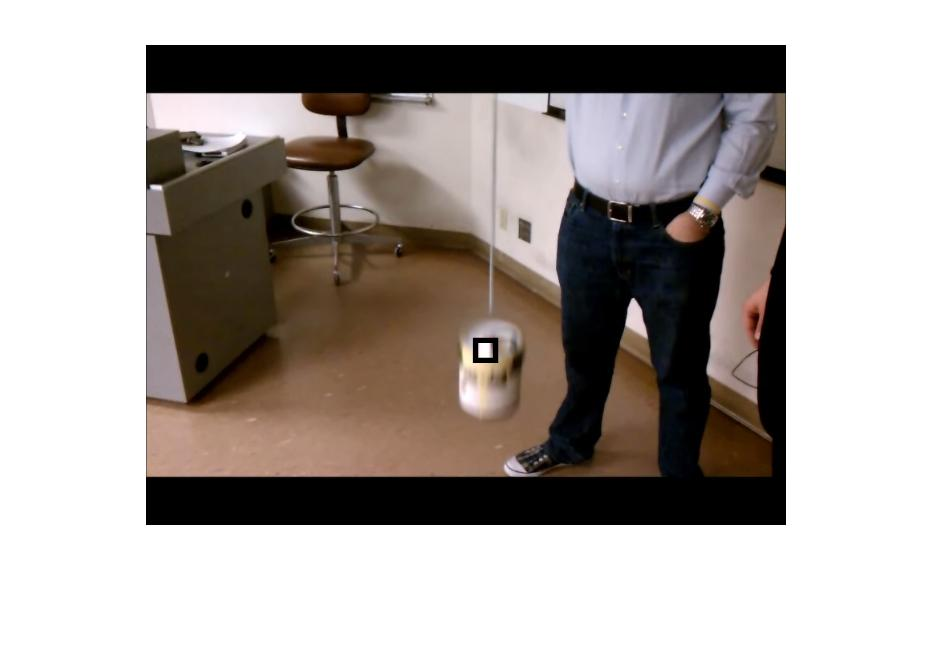
\includegraphics[width = 0.45\textwidth]{1example.jpg}
        \caption{A frame of light I found(black box)}
        \label{fig:example}
    \end{figure}

    Then for convenience of comparing and computing, I made all data I got to be in the same size (length). With this
    step, we could then compare the displacement on every direction. In the first test (ideal case), the displacement vs.
    time graph for both x-axis and y-axis I got is Figure \ref{fig:test1_1}
    \begin{figure}[h]
        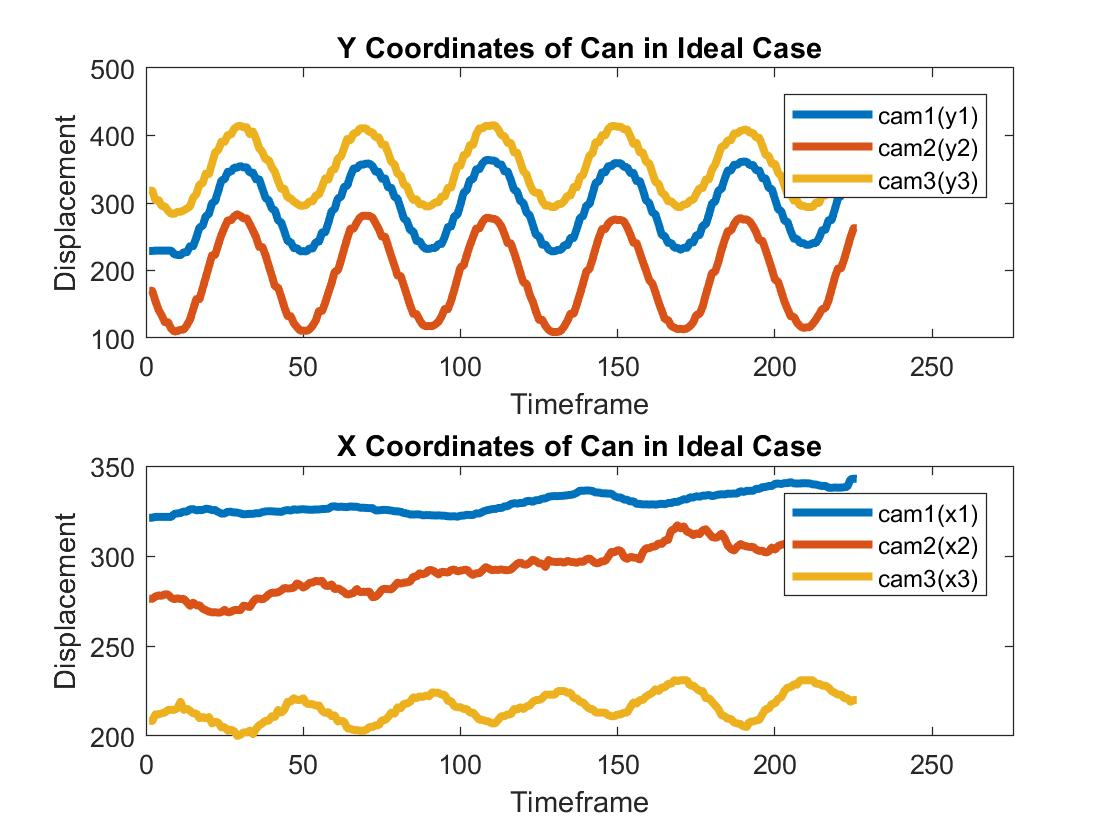
\includegraphics[width = 0.45\textwidth]{test1_1.jpg}
        \caption{Ideal Case, Dispalcement vs Time}
        \label{fig:test1_1}
    \end{figure}
    In order to have a better understanding on the differences of displacement among different cameras, I normalized the 
    displacement to have a more readable plot like Figure \ref{fig:test1_2}
    \begin{figure}[h]
        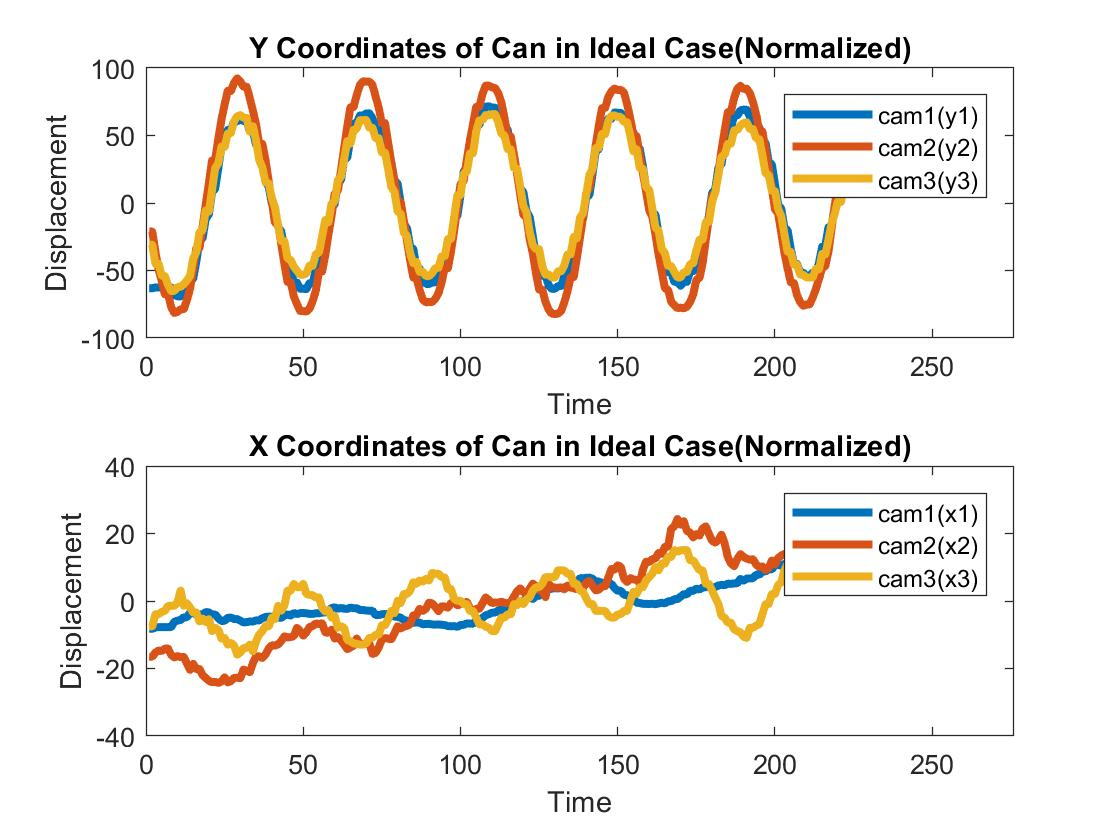
\includegraphics[width = 0.45\textwidth]{test1_2.jpg}
        \caption{Ideal Case, Dispalcement vs Time (Normalized)}
        \label{fig:test1_2}
    \end{figure}
    Then it is time to discuss how many directions are playing roles in this experiment. The most simple way is to proceed
    a singular value decomposition (SVD) and have a look at the diagonal matrix. With doing that, I got Figure 
    \ref{fig:test1_3} and conclude that there is only one direction mattering the phenomena. In the other word, it is a 
    1D motion.
    \begin{figure}[h]
        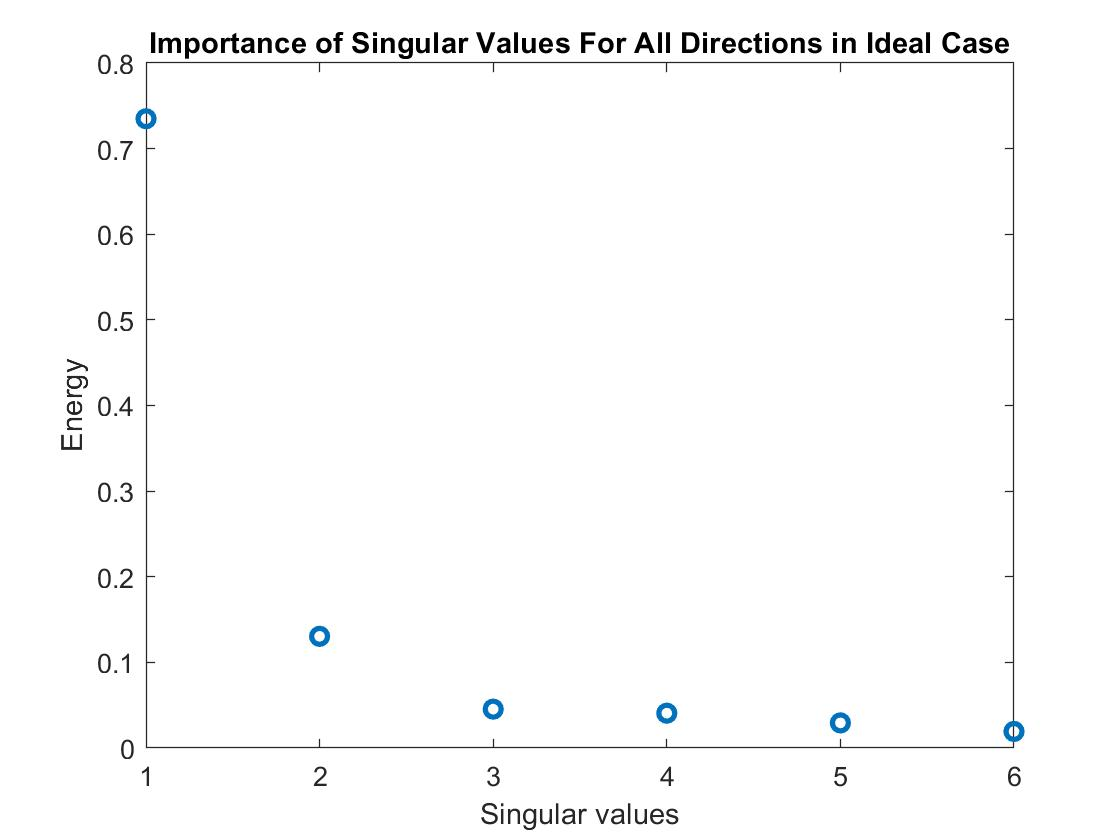
\includegraphics[width = 0.45\textwidth]{test1_3.jpg}
        \caption{Ideal Case, Importance of Each Direction}
        \label{fig:test1_3}
    \end{figure}

    Similarly, we could do the same analysis to other cases (noisy, horizontal displacement, horizontal dispalcement and rotation)
    \begin{figure}[h]
        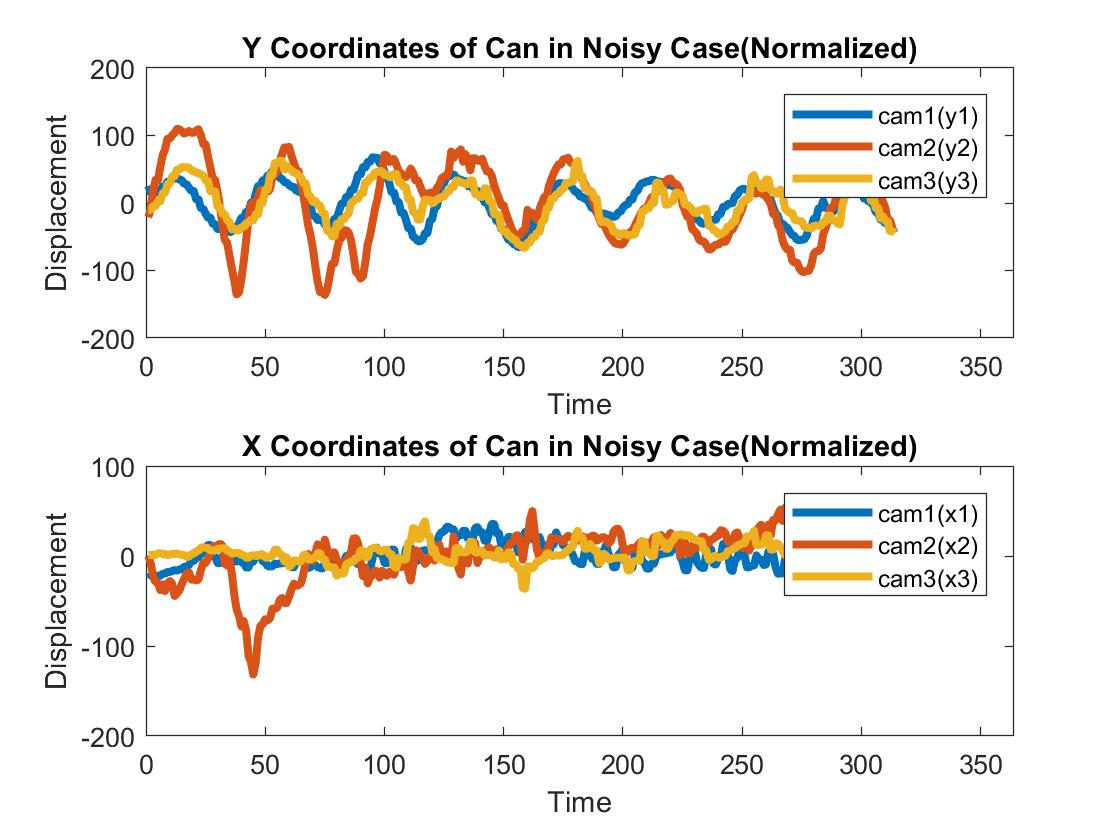
\includegraphics[width = 0.45\textwidth]{test2_1.jpg}
        \caption{Noisy Case, Dispalcement vs Time (Normalized)}
        \label{fig:test2_1}
    \end{figure}
    \begin{figure}[h]
        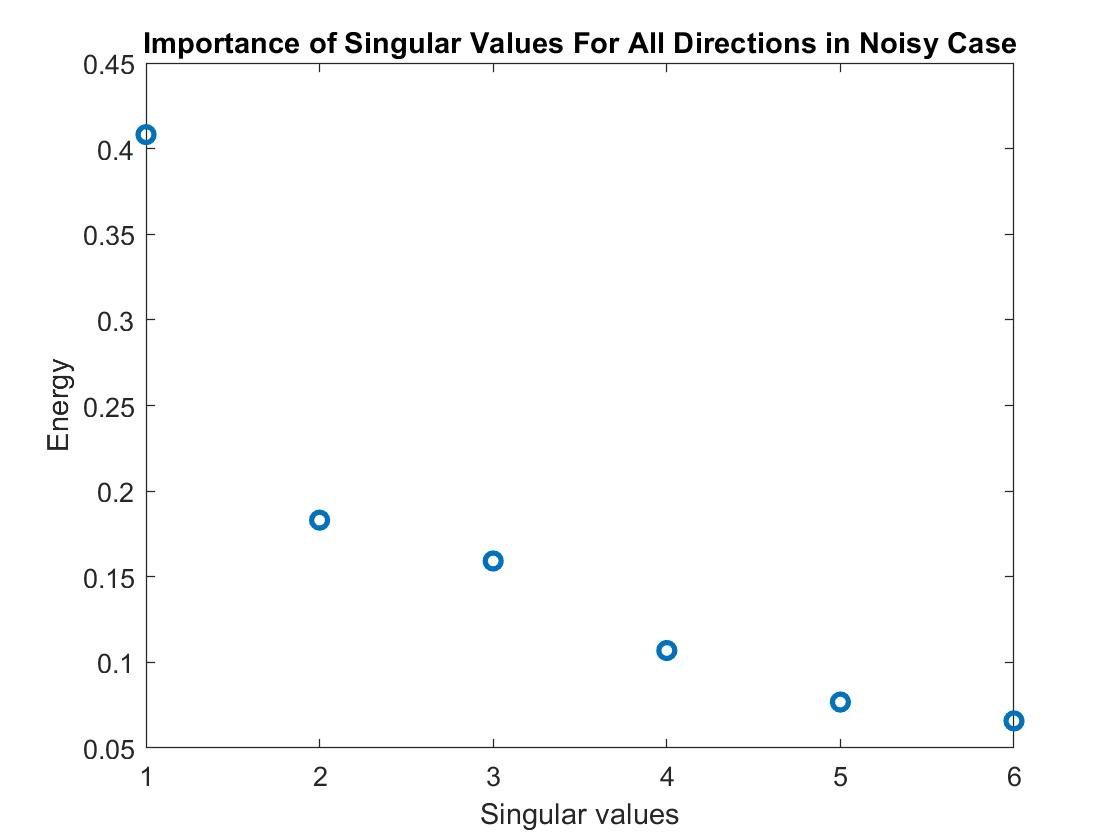
\includegraphics[width = 0.45\textwidth]{test2_2.jpg}
        \caption{Noisy Case, Importance of Each Direction}
        \label{fig:test2_2}
    \end{figure}
    \begin{figure}[h]
        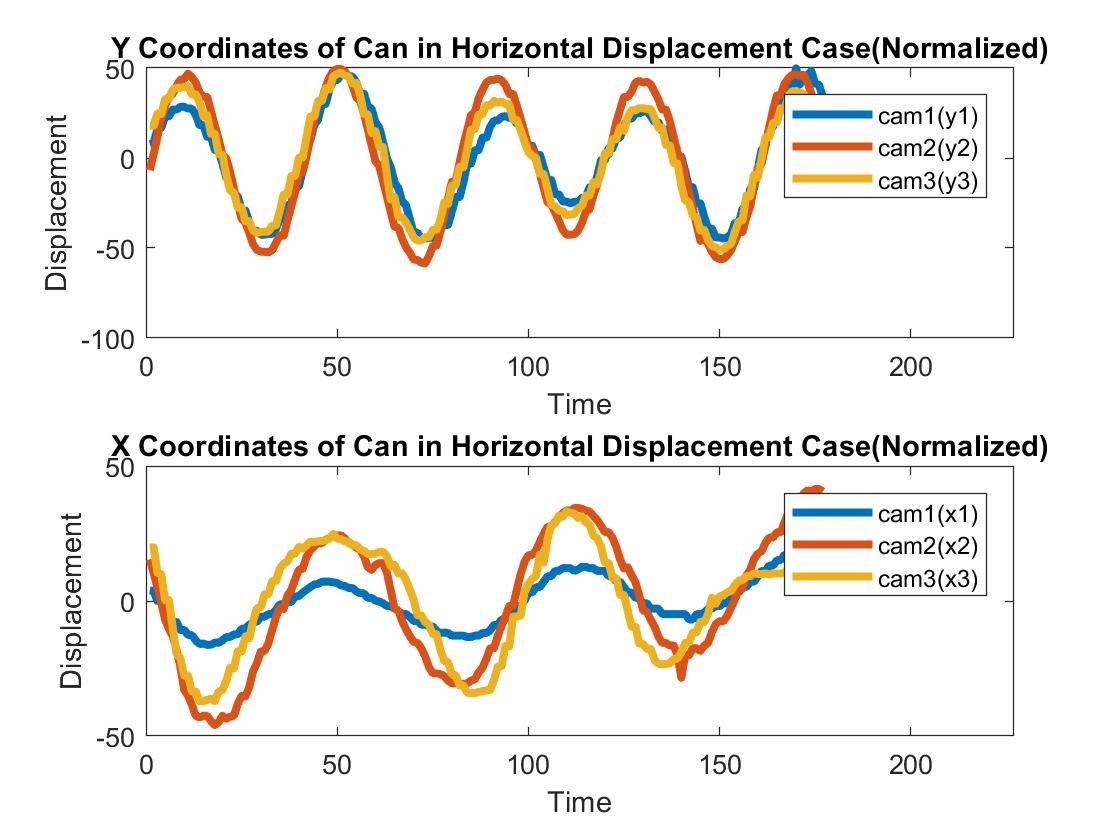
\includegraphics[width = 0.45\textwidth]{test3_1.jpg}
        \caption{Horizontal Case, Dispalcement vs Time (Normalized)}
        \label{fig:test3_1}
    \end{figure}
    \begin{figure}[h]
        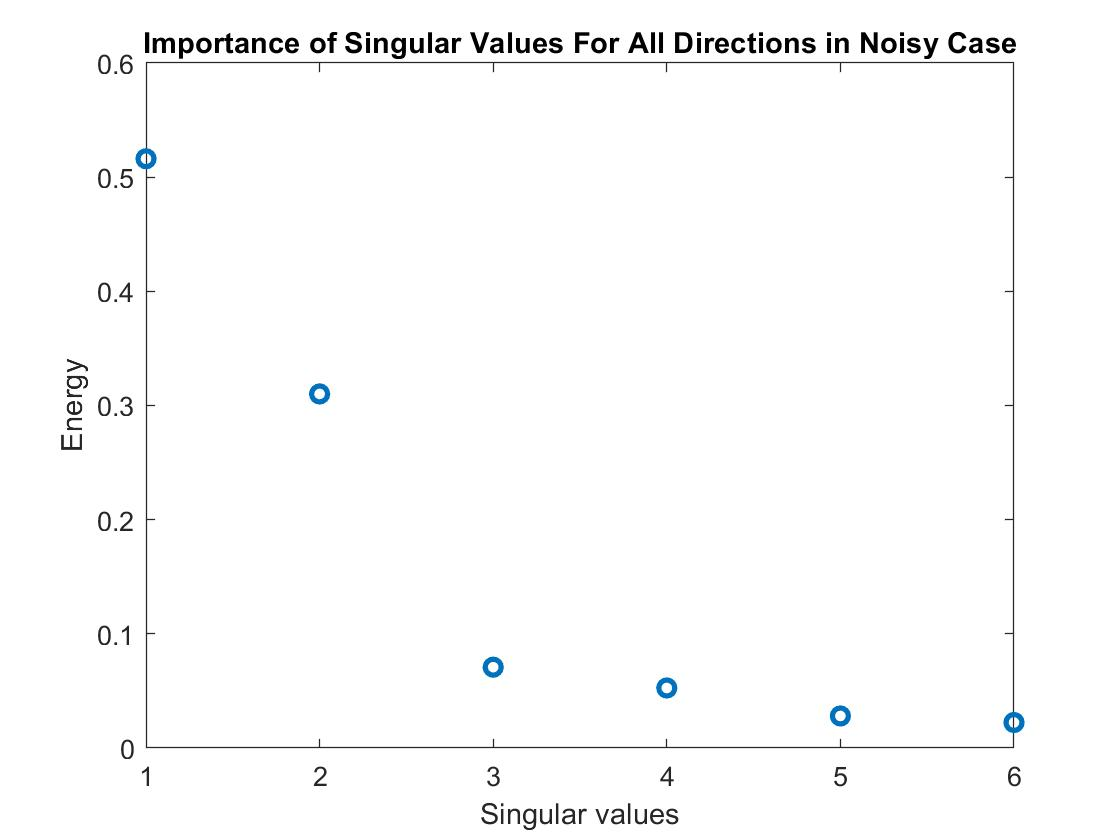
\includegraphics[width = 0.45\textwidth]{test3_2.jpg}
        \caption{Horizontal Case, Importance of Each Direction}
        \label{fig:test3_2}
    \end{figure}
    \begin{figure}[h]
        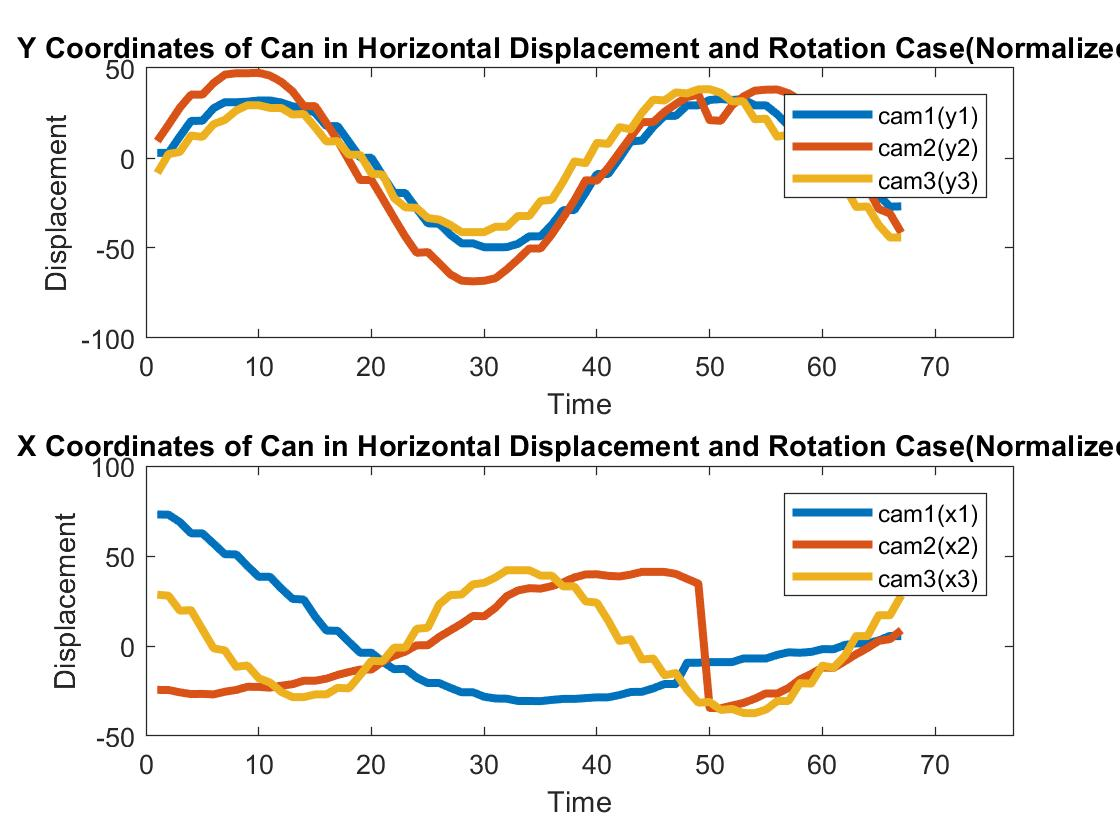
\includegraphics[width = 0.45\textwidth]{test4_1.jpg}
        \caption{Horizontal and Rotation Case, Dispalcement vs Time (Normalized)}
        \label{fig:test4_1}
    \end{figure}
    \begin{figure}[h]
        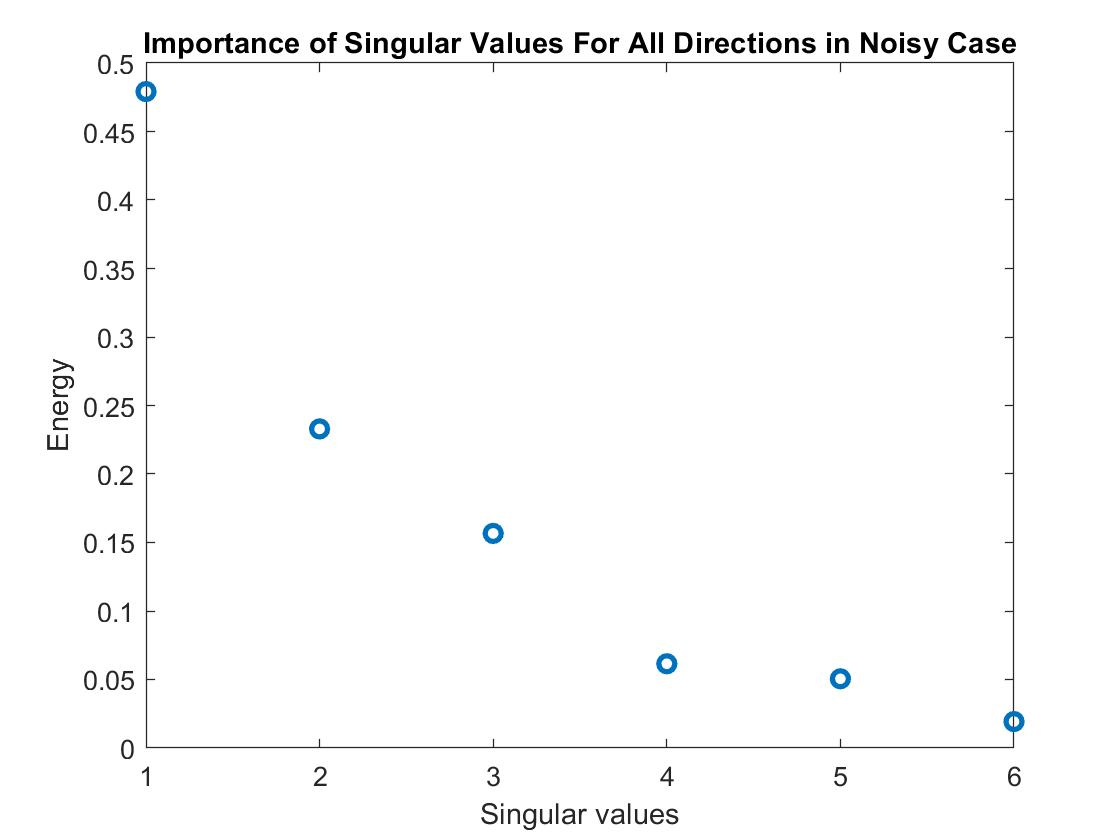
\includegraphics[width = 0.45\textwidth]{test4_2.jpg}
        \caption{Horizontal and Rotation Case, Importance of Each Direction}
        \label{fig:test4_2}
    \end{figure}
    From the graphs, we can see that the noisy data affects our determination a lot according to Figure \ref{fig:test2_1}.
    In this figure, the second camera has its curve that is kind of off-track due to noise. However, from the importance 
    graph (Figure \ref{fig:test2_2}), we can still conclude that there is only one single direction that matters since the
    other singular values has much lower importance (energy) comparing to the first singular value. \\
    And third test (horizontal displacement) results in that 2 directions play important roles in its motion, which make 
    sense since it moves horizonally (x-direction) and vertically (z-direction). We made the same conclusion due to Figure
    \ref{fig:test3_2}. And the last test is somehow tricky since there are two singular values that have values but not
    too big. I concluded that it is a 3D motion in test 4.

    \section{Summary and Conclusions}
    The Principal Component Analysis is useful and effective. Using this method, we are able to illustrate real-life
    phenomena from data perspective by simply reproduce the situation and study for it. However, it is very important to 
    elinimate noisy data as much as possible since noise will have huge effect during the process of analysis. It is okay
    to take redundant data since PCA will take out those by chaging the basis. But it is hard to detect noise and those noise
    will affect our conclusion.
    %----------------------------------------------------------------------------------------
    %	APPENDIX
    %----------------------------------------------------------------------------------------

    \mbox{~}
    \clearpage
    \begin{appendices}
    \setboolean{@twoside}{false}
    \setboolean{@twocolumn}{false}
        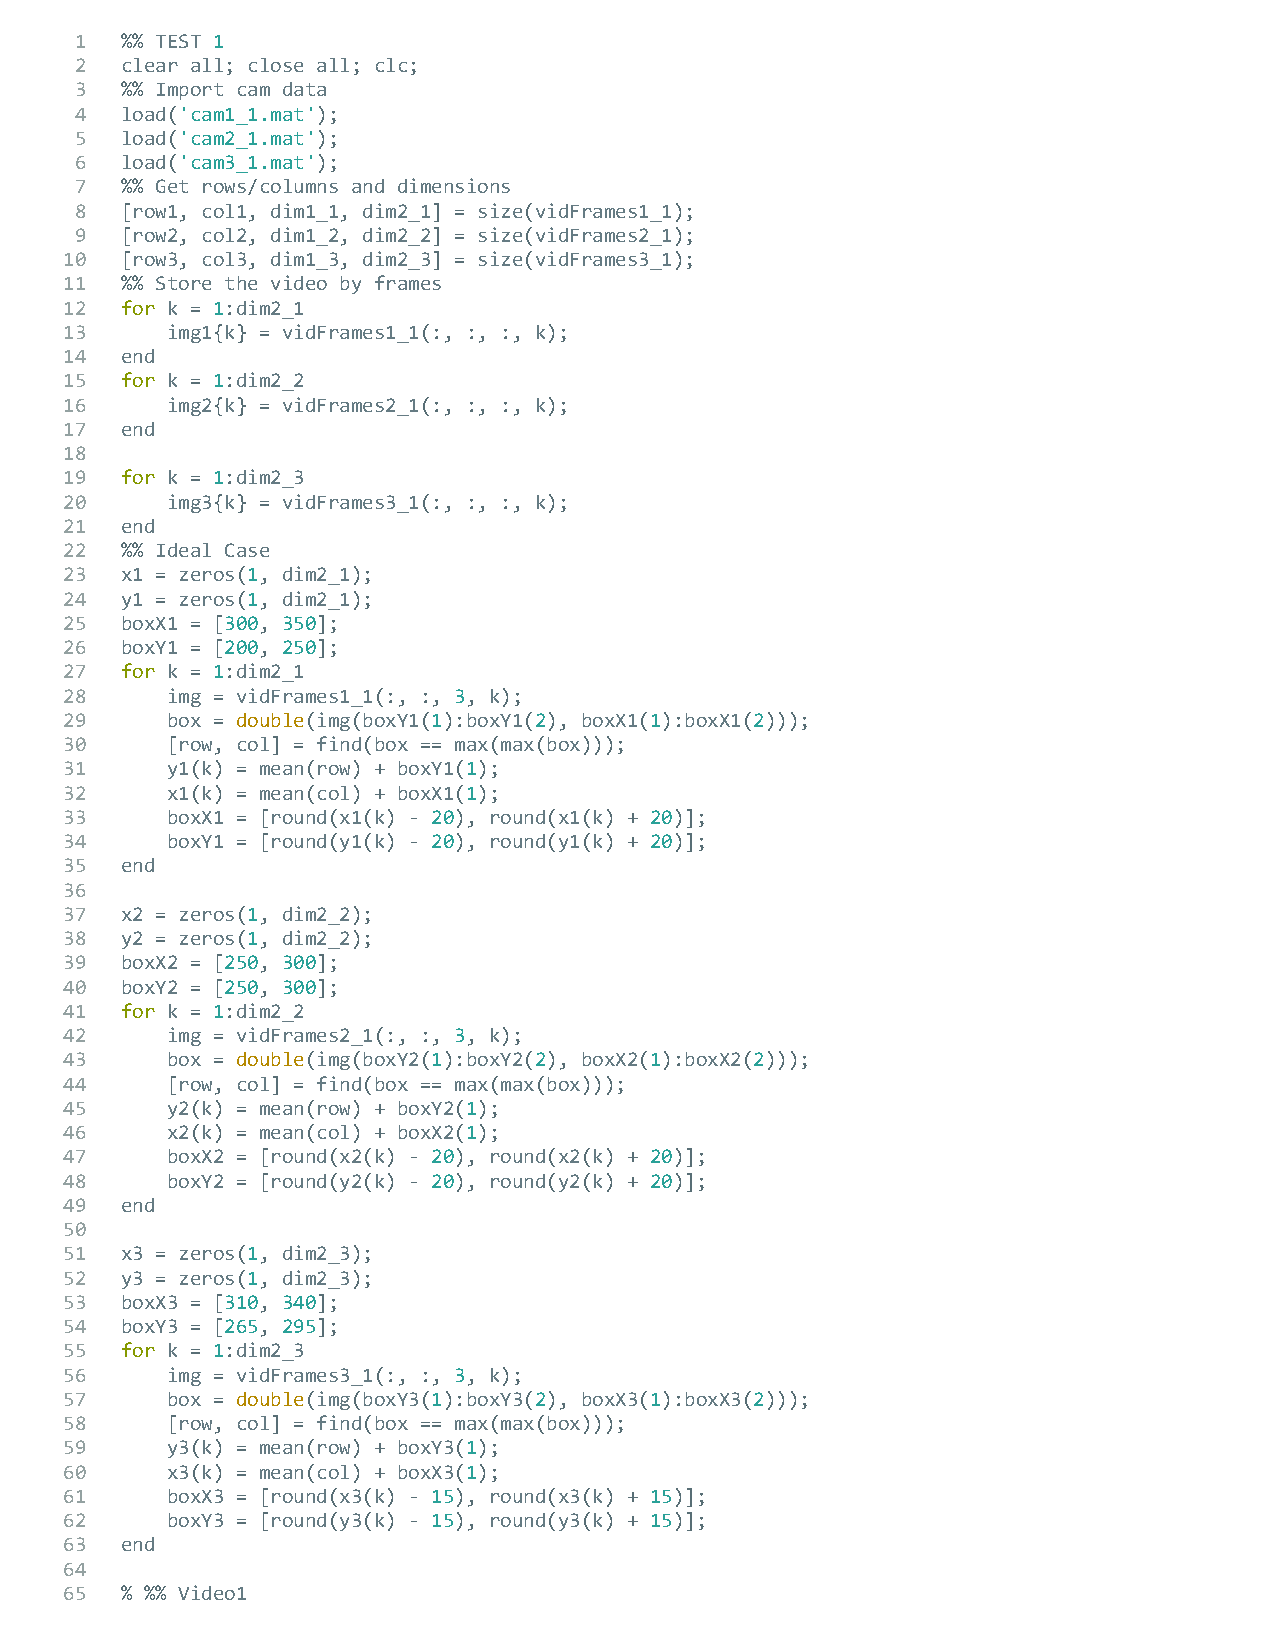
\includepdf[pages=-]{appendix.pdf}
    \end{appendices}

\end{document}